\documentclass{scrreprt}
\usepackage{listings}
\usepackage{underscore}
\usepackage{float}
\usepackage{graphicx}
\usepackage[bookmarks=true]{hyperref}
\usepackage[utf8]{inputenc}
\usepackage[spanish]{babel}
\usepackage{subfiles}
\usepackage{blindtext}


\hypersetup{
    bookmarks=false,    % show bookmarks bar?
    pdftitle={DOCUMENTO DE REQUISITOS},    % title
    pdfauthor={Grupo Rojo},                     % author
    pdfsubject={Compitational Learning},                        % subject of the document
    pdfkeywords={TeX, LaTeX, graphics, images}, % list of keywords
    colorlinks=true,       % false: boxed links; true: colored links
    linkcolor=black,       % color of internal links
    citecolor=black,       % color of links to bibliography
    filecolor=black,        % color of file links
    urlcolor=purple,        % color of external links
    linktoc=page            % only page is linked
}%
\def\myversion{2.3}
\date{}
%\title
\usepackage{hyperref}
\begin{document}

\begin{center}
    \rule{16cm}{5pt}\vskip1cm
    \begin{bfseries}
        \Huge{GESTOR DE TAREAS ROBOTS ASISTENCIALES}\\
        \vspace{1.5 cm}
        grupo rojo\\
        \vspace{1.5 cm}
        Ingeniería Web\\
        \vspace{1.5 cm}
        \LARGE{Versión \myversion}\\
        \vspace{1 cm}
        Realizado por: Alejandro Domínguez Recio \\
        Hugo Ávalos de Rorthais \\
        Rosario García Morales\\
        Laura Núñez Jiménez\\
        Jesús Aldana Martín \\
        \vspace{1 cm}
        Profesor : Javier Cámara Moreno\\
        \vspace{1 cm}
        \today\\
    \end{bfseries}
\end{center}

\tableofcontents

\chapter{Introducción}
La sanidad pública en muchos países se ve saturada por la alta demanda de pacientes enfermos o que requieren de un diagnóstico, esto provoca grandes retrasos a la hora de pedir citas y aumenta la probabilidad de que produzcan problemas humanos por el nivel de saturación que encontramos en algunos hospitales. Es por ello que los robots asistenciales están tomando mucho protagonismo en el ámbito sanitario. Estos pueden mejorar el rendimiento y optimizar trabajos para ayudar así al sanitario. Para mejorar está situación se han comenzado a incorporar en los hospitales robots controlados por una aplicación que ayuden a tener una mejor comunicación interna dentro del hospital y liberar a los sanitarios, enfermeros y auxiliares de tareas rutinarias que a día de hoy pueden resolver robots sin ningún tipo de problema. 

\section{Objetivos}
Durante el desarrollo de nuestra aplicación buscamos resolver los siguientes escenarios:
Con el desarrollo de este proyecto perseguimos crear una aplicación web que comunique de forma remota al sanitario con los robots del hospital, principalmente nos centraremos en la inserción y modificación de tareas desde la web. Para que el robot se desplace automáticamente tras recibir alguna petición por parte del sanitario. Los robots y, por tanto, nuestra app se centrara en tareas especializadas en desinfección, transporte de medicamentos y teleasistencia.

\begin{itemize}
    \item Permitir la comunicación entre el sanitario y el robot. 
    \item Una buena gestión de manejo de tareas de los robots asistenciales.
    \item Agilizar el trabajo del personal sanitario. 
\end{itemize}

\section{Formato utilizado}

Se ha decidido usar una tabla por requisito. En cada tabla se añadirá la descripción del requisito, la prioridad que tiene respecto a los demás, el riesgo de no cumplirse y una descripción del mismo, el motivo del requisito. Se implementa también una parte de criterios de aceptación para saber que el requisito ha sido implementado adecuadamente. Se utiliza la misma plantilla para FR y NFR, porque son requisitos como tal, y su estructura son parecidas. El motivo por el cual se ha decidido usar esta implementación es la sencillez de visualización tanto para los realizadores del proyecto como para el cliente a la hora de mostrarle estos requisitos, esto es más sencillo, debido a que los requisitos van a tener una estructura organizada y esquematizada. Cuando lo veamos ya sabemos directamente muchas funcionalidades del requisito.  



\chapter{Descripción de producto}
El producto trata de una aplicación web orientada a la gestión de robots de un centro sanitario. Esta aplicación por parte del sanitario se usará para gestionar los robots y obtener 'feedback' sobre su estado. Por parte del técnico, modificará la plantilla de robots, definirá los posibles comportamientos y tratará con los errores de los mismos.

\section{Características de los usuarios y entorno }

Definiendo como usuario a toda aquella persona que interactúa directamente con la aplicación. En esta sección se detallaran las principales características de los usuarios así como del uso que harán estos de la aplicación. 

\begin{table}[H]
\subsection{Resumen de los usuarios}
\vspace{0.3cm}
\label{tab:my-table-user}

\begin{tabular}{ |p{2cm}|p{10cm}|p{3cm}|  }
\hline
 \textbf{Nombre} & \textbf{Descripción} & \textbf{Relaciones}\\
\hline
Técnico                        & Encargado de la gestión técnica de la flota de robots. Realiza las tareas de incorporación o retirada de robots, configuración de tareas o apoya en caso de incidencias & Relación Técnico-Sanitario \\ 
\hline
Sanitario                          & Encargado de la gestión del estado de la flota de robots. Realiza las tareas de asignación, modificación o eliminación de las tareas asignadas a los robots. & Relación Sanitario-Técnico  \\ 
\hline
\end{tabular}%

\caption{Resumen usuarios}
\end{table}

\subsection{Perfiles de usuarios}
\vspace{0.3cm}
\begin{table}[H]
\label{tab:my-table-user}
\begin{tabular}{|p{4cm}|p{11cm}|}
\hline
\multicolumn{2}{|c|}{\textbf{TÉCNICO}} \\ \hline
\textbf{Representante}                         & Técnico.  \\ \hline
\textbf{Descripción} &  Persona con conocimientos técnicos sobre los robots. Aplica los conocimientos técnicos en la configuración, mantenimiento, reparación y solución de problemas de estos. \\ \hline
\textbf{Responsabilidades}                         &  • Incorporar o retirar robots de la flota \\
 &  •	Definir el conjunto de tareas permitidas en los robots (Dentro de su tipo). \\
 & •	Modificar características técnicas de los robots (Ej : Modo energía )  \\ 
 & •	Asistir incidencias técnicas \\
 \hline
\textbf{Criterio de éxito}                         & Proporcionar un sistema que cubra sus responsabilidades de una forma simple.  \\ \hline
\end{tabular}%

\caption{Tabla Usuario_1}
\end{table}

\begin{table}[H]
\label{tab:my-table-user}
\begin{tabular}{|p{4cm}|p{11cm}|}
\hline
\multicolumn{2}{|c|}{\textbf{SANITARIO}} \\ \hline
\textbf{Representante}                         & Sanitario.  \\ \hline
\textbf{Descripción} &  Persona con conocimientos sobre tratamientos o cuidados aplicados a la salud de las personas. Identifica, realiza y requiere de actividades aplicadas en su práctica clínica. \\ \hline
\textbf{Responsabilidades}                         &  •	Asignar tareas a los robots. \\
 &  •	Fijar prioridad a las tareas. \\
 &  •	Fijar tiempo de realización a las tareas \\ 
 &  •	Modificar estado de tareas. \\
 &  •	Revisar estado de los robots y tareas asociadas \\
 \hline
\textbf{Criterio de éxito}                         & Proporcionar un sistema que cubra sus responsabilidades de una forma simple.  \\ \hline
\end{tabular}%

\caption{Tabla Usuario_2}
\end{table}

\section{Funcionalidad del producto}
El producto mejorará la organización de tareas de un conjunto de robots. Este implementará una app donde tenga una interfaz orientativa para el médico y así se obtenga una buena comunicación con los robots. 
\newline


\chapter{Requisitos funcionales}
A continuación los requisitos funcionales desarrollados para la aplicación. Cada tabla corresponde a un requisito diferente cada requisito es nombrado por un identificador único, en nuestro caso se trata de "FR\_NúmeroRequisito" y cada fila de la tabla revela información adicional sobre el requisito en cuestión.
\\

\section{Requisitos funcionales}

\subsection{FR 0}

\begin{table}[H]
    \label{tab:my-table}
    \begin{tabular}{|p{5cm}|p{11cm}|}
    \hline
    \multicolumn{2}{|c|}{\textbf{FR_0}} \\
    \hline
    \textbf{Descripción  }                      & El técnico podrá incorporar y eliminar usuarios de la apliación  \\ \hline
    \textbf{Prioridad}                          & Alta \\ \hline
    \textbf{Riesgo}                          & Nulo \\ \hline
    \textbf{Descripción del riesgo}                    & Nulo  \\ \hline
    \textbf{Razón}                   & Proporcionar funcionalidad de gestión básica al técnico  \\ \hline
    \textbf{Criterio de aceptación}                    & El usuario nuevo aparece en la base de datos  \\ \hline
    \end{tabular}%
    \caption{Requisito Funcional FR_0}
\end{table}

\subsection{FR 1}
\begin{table}[H]
    \label{tab:my-table}
    
    \begin{tabular}{|p{5cm}|p{11cm}|}
    \hline
    \multicolumn{2}{|c|}{\textbf{FR_1}} \\
    \hline
    \textbf{Descripción  }                      & El técnico podrá definir el conjunto de tareas permitidas en los robots                                                                                            \\ \hline
    \textbf{Prioridad}                          & Alta                                                                                              \\ \hline
    \textbf{Riesgo}                          & Nulo                                                                                                \\ \hline
    \textbf{Descripción del riesgo}                    & Nulo                                                                               \\ \hline
    \textbf{Razón}                   & Proporcionar funcionalidad de gestión básica al técnico                                                                                                 \\ \hline
    \textbf{Criterio de aceptación}                    & La tarea aparecerá en la vitsa de lista de tareas \\ \hline

    \end{tabular}%
    
    \caption{Requisito Funcional FR_1}
\end{table}


\subsection{FR 2}
    \begin{table}[H]
    
    \label{tab:my-table}
    
    \begin{tabular}{|p{5cm}|p{11cm}|}
    \hline
    \multicolumn{2}{|c|}{\textbf{FR_2}} \\
    \hline
    \textbf{Descripción  }                      & El técnico puede ver la asistencias de problemas técnicos.                                                                             \\ \hline
    \textbf{Prioridad}                          & Alta                                                                                              \\ \hline
    \textbf{Riesgo}                          & Nulo                                                                                                \\ \hline
    \textbf{Descripción del riesgo}                    & Nulo                                                                               \\ \hline
    \textbf{Razón}                   & Proporcionar funcionalidad de atención técnica a los sanitarios.                                                                                               \\ \hline
    \textbf{Criterio de aceptación}                    &  Las incidencias aparecen en la ventana de incidencias \\ \hline
    \end{tabular}%
    
    \caption{Requisito Funcional RF_2}
\end{table}

\subsection{FR 3}
\begin{table}[H]
    \label{tab:my-table}
    
    \begin{tabular}{|p{5cm}|p{11cm}|}
    \hline
    \multicolumn{2}{|c|}{\textbf{FR_3}} \\
    \hline
    \textbf{Descripción  }                      & El sistema debe posibilitar al técnico la monitorización de robots                                                                            \\ \hline
    \textbf{Prioridad}                          & Alta                                                                                              \\ \hline
    \textbf{Riesgo}                          & Nulo                                                                                                \\ \hline
    \textbf{Descripción del riesgo}                    & Nulo                                                                               \\ \hline
    \textbf{Razón}                   & Proporcionar funcionalidad de gestión básica al técnico. La monitorización de los distintos robots es clave a la hora planificar o asignar tareas.                                                                                                \\ \hline
    \textbf{Criterio de aceptación}                    &   \\ \hline
    \end{tabular}%
    
    \caption{Requisito Funcional RF_3}
\end{table}

\subsection{FR 4}
    \begin{table}[H]
        \label{tab:my-table}
        \begin{tabular}{|p{5cm}|p{11cm}|}
        \hline
        \multicolumn{2}{|c|}{\textbf{FR_4}} \\
        \hline
        \textbf{Descripción  }                      &  El sanitario dispondrá de una herramienta de filtrado para los robots.                                                                       \\ \hline
        \textbf{Prioridad}                          & Media                                                                                              \\ \hline
        \textbf{Riesgo}                          & Medio                                                                                                \\ \hline
        \textbf{Descripción del riesgo}                    & Filtración de los robots de manera desordenada o que esten en un estado que no es el correspondiente                        \\ \hline
        \textbf{Razón}                   & Facilitar la navegación del sanitario                                                                                                                \\ \hline
        \textbf{Criterio de aceptación}                    & El filtrado será correspondiente a cada estado del robot.  \\ \hline
        \end{tabular}%
        
        \caption{Requisito Funcional RF_4}
\end{table}


\subsection{FR 5}
\begin{table}[H]

    \label{tab:my-table}
    
    \begin{tabular}{|p{5cm}|p{11cm}|}
    \hline
    \multicolumn{2}{|c|}{\textbf{FR_5}} \\
    \hline
    \textbf{Descripción  }                      &  El sanitario podrá asignar tareas.                                                                           \\ \hline
    \textbf{Prioridad}                          & Máxima                                                                                              \\ \hline
    \textbf{Riesgo}                          & Máximo                                                                                                \\ \hline
    \textbf{Descripción del riesgo}                    & Toda la aplicación gira entorno a la asignación de tareas del sanitario al robot.                                                                          \\ \hline
    \textbf{Razón}                   & Al guardar las tareas en una cola tendremos organizadas las tareas a realizar.                                                                                              \\ \hline
    \textbf{Criterio de aceptación}                    & Asignación de tarea correcta y aparezca en la lista de tareas del robot.  \\ \hline
    \end{tabular}%
    
    \caption{Requisito Funcional RF_5}
\end{table}

\subsection{FR 6}
    \begin{table}[H]
    
    \label{tab:my-table}
    
    \begin{tabular}{|p{5cm}|p{11cm}|}
    \hline
    \multicolumn{2}{|c|}{\textbf{FR_6}} \\
    \hline
    \textbf{Descripción  }                      & El sanitario tendrá la posibilidad de dar diferentes niveles de prioridad.                                                                            \\ \hline
    \textbf{Prioridad}                          & Máxima                                                                                              \\ \hline
    \textbf{Riesgo}                          & Máximo                                                                                                \\ \hline
    \textbf{Descripción del riesgo}                    & Que hayan tareas urgentes en lista de espera y no se realicen antes que las otras.                                                                           \\ \hline
    \textbf{Razón}                   & Los robots tienen que hacer las tareas urgentes antes que las demás.A más alta automáticamente se colocarán por encima de otras más triviales en la cola.                                                                                        \\ \hline
     \textbf{Criterio de aceptación}                    & Asignación de tarea correcta y aparezca en la lista de tareas del robot como la primera.  \\ \hline
    \end{tabular}%
    
    \caption{Requisito Funcional RF_6}
\end{table}



\subsection{FR 7}
\begin{table}[H]
    
    \label{tab:my-table}
    
    \begin{tabular}{|p{5cm}|p{11cm}|}
    \hline
    \multicolumn{2}{|c|}{\textbf{FR_7}} \\
    \hline
    \textbf{Descripción  }                      & Las tareas de prioridad ‘Máxima’ interrumpirán la tarea que esté desempeñando el robot para el cumplimiento de la misma.                                                                          \\ \hline
    \textbf{Prioridad}                          & Alta                                                                                              \\ \hline
    \textbf{Riesgo}                          & Nulo                                                                                                \\ \hline
    \textbf{Descripción del riesgo}                    & Nulo                                                                               \\ \hline
    \textbf{Razón}                   & Proporcionar funcionalidad de gestión básica del sistema.                                                                                               \\ \hline
     \textbf{Criterio de aceptación}                    & La tarea de urgencia maxima aparece la primera en el listado de tareas.  \\ \hline
\end{tabular}%

\caption{Requisito Funcional RF_7}
\end{table}

\subsection{FR 8}
    \begin{table}[H]
    
    \label{tab:my-table}
    
    \begin{tabular}{|p{5cm}|p{11cm}|}
    \hline
    \multicolumn{2}{|c|}{\textbf{FR_8}} \\
    \hline
    \textbf{Descripción  }                      & Las tareas interrumpidas se reasignan/eliminan de la cola según su prioridad
                                                                             \\ \hline
    \textbf{Prioridad}                          & Alta                                                                                              \\ \hline
    \textbf{Riesgo}                          & Medio                                                                                                \\ \hline
    \textbf{Descripción del riesgo}                    & Que no aparezcan en la lista o que sigan apareciendo. Haría que entrará en bucle la lista de tareas.                                                                              \\ \hline
    \textbf{Razón}                   & Proporcionar funcionalidad de gestión básica del sistema.                                                                                               \\ \hline
     \textbf{Criterio de aceptación}                    & Las tareas interrumpidas se hayan eliminado del historial del robot.  \\ \hline
    \end{tabular}%
    
    \caption{Requisito Funcional RF_8}
\end{table}

\subsection{FR 9}
\begin{table}[H]
    \label{tab:my-table}
    \begin{tabular}{|p{5cm}|p{11cm}|}
    \hline
    \multicolumn{2}{|c|}{\textbf{FR_9}} \\
    \hline
    \textbf{Descripción  }                      &  La aplicación debe tener registro e inicio de sesión.                                                                       \\ \hline
    \textbf{Prioridad}                          & Alta                                                                                              \\ \hline
    \textbf{Riesgo}                          & Alto                                                                                                \\ \hline
    \textbf{Descripción del riesgo}                    & No saber a que funcionalidad dar acceso.                                                                \\ \hline
    \textbf{Razón}                   & Debemos conocer en todo momento que usuarios acceden a la app.                                                                                             \\ \hline
     \textbf{Criterio de aceptación}                    & El usuario entrará en su interfaz correspondiente.  \\ \hline
    \end{tabular}%
    
    \caption{Requisito Funcional RF_9}
\end{table}

\subsection{FR 10}
    \begin{table}[H]
        \label{tab:my-table}
        \begin{tabular}{|p{5cm}|p{11cm}|}
        \hline
        \multicolumn{2}{|c|}{\textbf{FR_10}} \\
        \hline
        \textbf{Descripción  }                      &  Toda los datos que genere la app serán recogidos y almacenados.                                                                      \\ \hline
        \textbf{Prioridad}                          & Alta                                                                                              \\ \hline
        \textbf{Riesgo}                          & Medio                                                                                                \\ \hline
        \textbf{Descripción del riesgo}                    &  Perder información que puede ser valiosa o necesaria para la app.                                \\ \hline
        \textbf{Razón}                   & Por motivos de seguridad guardaremos la información de quien ha tenido acceso a la app.                                                                                                                \\ \hline
         \textbf{Criterio de aceptación}                    & Asignación de tarea correcta y aparezca en la lista de tareas del robot.  \\ \hline
        \end{tabular}%
        
        \caption{Requisito Funcional RF_10}
\end{table}

\subsection{FR 11}
    \begin{table}[H]
        \label{tab:my-table}
        \begin{tabular}{|p{5cm}|p{11cm}|}
        \hline
        \multicolumn{2}{|c|}{\textbf{FR_11}} \\
        \hline
        \textbf{Descripción  }                      &  Debe haber un registro de todas las tareas hecha por cada robot                                              \\ \hline
        \textbf{Prioridad}                          & Alta                                                                                              \\ \hline
        \textbf{Riesgo}                          & Bajo                                                                                                \\ \hline
        \textbf{Descripción del riesgo}                    &  Perder información que puede ser valiosa o necesaria para la app.                                \\ \hline
        \textbf{Razón}                   & Por motivos de seguridad guardaremos la información de que ha hecho cada robot, en que momento y quien se lo ha ordenado.                                                                                                      \\ \hline
         \textbf{Criterio de aceptación}                    & En el listado de tareas tanto para el sanitario como para el técnico aparezcan todas las tareas propuestas.  \\ \hline
        \end{tabular}%
        
        \caption{Requisito Funcional RF_11}
\end{table}

\chapter{Requisitos no funcionales}

\section{Requisitos de almacenamiento}

\subsection{NFR 0}
\begin{table}[H]
    \label{tab:my-table}
    \begin{tabular}{|p{5cm}|p{11cm}|}
    \hline
    \multicolumn{2}{|c|}{\textbf{NFR_0}} \\
    \hline
    \textbf{Descripción  }                      &  Se utilizarán herramientas de almacenamiento en la nube para guardar los datos de la app.                                                                            \\ \hline
    \textbf{Prioridad}                          & Media                                                                                              \\ \hline
    \textbf{Riesgo}                          & Medio                                                                                                \\ \hline
    \textbf{Descripción del riesgo}                    & Perder información valiosa.                                                                               \\ \hline
    \textbf{Razón}                   & Los datos en la nube están más seguros que en local.                                                                                               \\ \hline
    \textbf{Padres}                               &  FR_10\\  \hline
     \textbf{Criterio de aceptación}                    & Todos los datos apareceran en la nube  \\ \hline
    \end{tabular}%
    
    \caption{Requisito No Funcional NRF_0}
\end{table}

\subsection{NFR 1}
\begin{table}[H]
    \label{tab:my-table}
    \begin{tabular}{|p{5cm}|p{11cm}|}
    \hline
    \multicolumn{2}{|c|}{\textbf{NFR_1}} \\
    \hline
    \textbf{Descripción  }                      &  El tiempo de carga de página web deberá de ser menor a 2s                                 \\ \hline
    \textbf{Prioridad}                          & Alta                                                                                             \\ \hline
    \textbf{Riesgo}                          & Bajo                                                                                               \\ \hline
    \textbf{Descripción del riesgo}                    & Incompatibilidad con características de diseño                                 \\ \hline
    \textbf{Razón}                   & El tiempo de carga es fundamental en la experiencia de usuario                                                                                \\ \hline
    \textbf{Padres}                               &  NFR_2\\  \hline
     \textbf{Criterio de aceptación}                    & El tiempo estimado fue de 2 segundos o menos.  \\ \hline
    \end{tabular}%
    
    \caption{Requisito No Funcional NRF_1}
\end{table}

\section{Requisitos de seguridad}

\subsection{NFR 2}
    \begin{table}[H]
        \label{tab:my-table}
        \begin{tabular}{|p{5cm}|p{11cm}|}
        \hline
        \multicolumn{2}{|c|}{\textbf{NFR_2}} \\
        \hline
        \textbf{Descripción  }                      &  A la hora del registro, el usuario debe especificar si es sanitario o técnico                                                                      \\ \hline
        \textbf{Prioridad}                          & Alta                                                                                              \\ \hline
        \textbf{Riesgo}                          & Alto                                                                                                \\ \hline
        \textbf{Descripción del riesgo}                    &  De no ser así, no podríamos diferenciar entre clínico o técnico.                          \\ \hline
        \textbf{Razón}                   & Ambos tipos de usuario podrían acceder a las funciones del otro.                                                                                                                       \\ \hline
        \textbf{Padres}                               &  FR_9\\  \hline
         \textbf{Criterio de aceptación}                    & El usuario si tiene acceso correspondiente a su cargo le saldrá la interfaz adecuada  \\ \hline
        \end{tabular}%
        
        \caption{Requisito No Funcional NRF_2}
\end{table}

\subsection{NFR 3}
    \begin{table}[H]
        \label{tab:my-table}
        \begin{tabular}{|p{5cm}|p{11cm}|}
        \hline
        \multicolumn{2}{|c|}{\textbf{NFR_3}} \\
        \hline
        \textbf{Descripción  }                      &  Tras un registro la contraseña sera encriptada para guardarla como un id único y no tener acceso a ella.                                                                      \\ \hline
        \textbf{Prioridad}                          & Baja                                                                                              \\ \hline
        \textbf{Riesgo}                          & Medio                                                                                                \\ \hline
        \textbf{Descripción del riesgo}                    &  Acceder a los datos privados de nuestros usuarios.                          \\ \hline
        \textbf{Razón}                   & Para no tener en ningún momento acceso a las contraseñas de los usuarios.  \\ \hline
        \textbf{Padres}                               &  FR_9\\  \hline
         \textbf{Criterio de aceptación}                    & Aviso de contraseña encriptada  \\ \hline
        \end{tabular}%
        
        \caption{Requisito No Funcional RNF_3}
\end{table}


\subsection{NFR 4}
    \begin{table}[H]
        \label{tab:my-table}
        \begin{tabular}{|p{5cm}|p{11cm}|}
        \hline
        \multicolumn{2}{|c|}{\textbf{NFR_4}} \\
        \hline
        \textbf{Descripción  }                      &  El sistema deberá de mantener un registro de usuario/clave única.                                                                    \\ \hline
        \textbf{Prioridad}                          & Alta                                                                                              \\ \hline
        \textbf{Riesgo}                          & Bajo                                                                                                \\ \hline
        \textbf{Descripción del riesgo}                    &  Funcionalidad de clave única proporcionada por la base de datos implementada                          \\ \hline
        \textbf{Razón}                   & Controlar el acceso a cuentas, como la identidad única de los usuarios.                                                                                         \\ \hline
        \textbf{Padres}                               &  FR_9\\  \hline
         \textbf{Criterio de aceptación}                    & Si el técnico añade un usuario le saldrá un aviso de que el usuario no existe en la base de datos, y podrá utilizar ese ID.  \\ \hline
        \end{tabular}%
        
        \caption{Requisito No Funcional NFR_4}
\end{table}

\section{Requisitos de diseño}

\subsection{NFR 5}
\begin{table}[H]
    \label{tab:my-table}
    \begin{tabular}{|p{5cm}|p{11cm}|}
    \hline
    \multicolumn{2}{|c|}{\textbf{NFR_5}} \\
    \hline
    \textbf{Descripción  }                      &  La web debe tener un diseño accesible y simple.                                                                            \\ \hline
    \textbf{Prioridad}                          & Alta                                                                                              \\ \hline
    \textbf{Riesgo}                          & Alto                                                                                                \\ \hline
    \textbf{Descripción del riesgo}                    & Que un sanitario sin ningún background tecnológico no sepa como trabajar con la app.                                                                               \\ \hline
    \textbf{Razón}                   & La app debe de ser auto explicativa para que cualquier usuario sepa utilizarla.       \\ \hline
    \textbf{Padres}                               &  FR_10\\  \hline
     \textbf{Criterio de aceptación}                    & La buena facilidad de manjera la aplicación.  \\ \hline
    \end{tabular}%
    
    \caption{Requisito No Funcional NRF_5}
\end{table}

\subsection{NFR 6}
    \begin{table}[H]
        \label{tab:my-table}
        \begin{tabular}{|p{5cm}|p{11cm}|}
        \hline
        \multicolumn{2}{|c|}{\textbf{NFR_6}} \\
        \hline
        \textbf{Descripción  }                      &  Según el tipo de usuario, la app tendrá una u otra interfaz.                                                                      \\ \hline
        \textbf{Prioridad}                          & Alta                                                                                              \\ \hline
        \textbf{Riesgo}                          & Medio                                                                                                \\ \hline
        \textbf{Descripción del riesgo}                    &  De no ser así, no podríamos diferenciar entre clínico o técnico.                          \\ \hline
        \textbf{Razón}                   & Ambos tipos de usuario podrían acceder a las funciones del otro.                                                                                                                       \\ \hline
        \textbf{Padres}                               &  FR_9\\  \hline
         \textbf{Criterio de aceptación}                    & La interfaz correspondiente a cada usuario.  \\ \hline
        \end{tabular}%
        
        \caption{Requisito No Funcional NFR_6}
\end{table}

\subsection{NFR 7}
    \begin{table}[H]
        \label{tab:my-table}
        \begin{tabular}{|p{5cm}|p{11cm}|}
        \hline
        \multicolumn{2}{|c|}{\textbf{NFR_7}} \\
        \hline
        \textbf{Descripción  }                      &  El sistema debe posibilitar la creación de una tarea con X clicks desde la vista monitorización del usuario                                                                      \\ \hline
        \textbf{Prioridad}                          & Alta                                                                                              \\ \hline
        \textbf{Riesgo}                          & Baja                                                                                                \\ \hline
        \textbf{Descripción del riesgo}                    &  Dificultad de crear lógica de procesos.                          \\ \hline
        \textbf{Razón}                   & La creación de tareas de una forma 'rápida' es fundamental en la experiencia de usuario. Se tiene en cuenta que la creación de tareas es una función principal de la aplicación                                                                                        \\ \hline
         \textbf{Criterio de aceptación}                    & Asignación de tarea correcta y fácil.  \\ \hline
        \end{tabular}%
        
        \caption{Requisito No Funcional NFR_7}
\end{table}

\chapter{Diseño}

El modelado web es una rama de la ingeniería web que aborda los problemas específicos relacionado con el diseño y desarrollo. En particular, se centra en el proceso de documentar un diseño de un sistema software complejo en un diagrama de flujo de estados de fácil comprensión utilizando texto y símbolos para representar la forma en la que el usuario accederá a la aplicación. Encontramos varios enfoques para el modelado web:

\begin{itemize}
    \item Modelo de procesos: Es una expresión abstracta de los procesos principales de un sistema se representa de manera secuencial.
    \item Diagramas IFML: Representa los elementos de la interfaz gráfica de la aplicación así como la forma en que el usuario pasa de un elemento a otro.
    \item Modelo  de contenidos:  Proporcionan una visión orientada a la ejecución, dan al desarrollador información a nivel de sistema.
\end{itemize}

Para tener una idea de como íbamos a realizar los diferentes modelos utilizamos una herramienta de dibujo para crear un boceto en el que mostramos de forma simple y mediante símbolos lo que contendrán en un futuro las diferentes vistas.

\begin{figure}[H]
	\centering
	\includegraphics[width=0.67\textwidth]{images/boceto_diseño.jpeg}
	\caption{Boceto inicial}
	\label{fig:example1}
\end{figure}

\section{Modelado de procesos}

El modelado de procesos es una expresión abstracta de los principales procesos de un sistema, y se suelen representar de manera secuencial. En los procesos se describe en que orden un grupo de objetos funcionan entre sí son utilizados para comprender mejor los requisitos de un sistema nuevo que se implemente o un proceso existente ya que nos permite visualizar de forma gráfica como se realizaran diferentes funcionalidades de la web. \\
\\
Dado que nuestra app presenta dos tipos de usuarios muy diferenciados hemos creado un proceso para cada uno de ellos en los que se muestra todas las opciones que tiene disponible y sus funcionalidades.\\
\\

\subsection{Técnico}

Cuando el usuario entra a la app web, el usuario se encuentra un login procede a poner usuario y contraseña, se confirma que el usuario está en la base de datos y entra a la interfaz correspondiente. El usuario puede volver al login o ir a lista de usuarios o tareas, donde desde el botón de usuario puede eliminar o añadir, y en la lista puede añadir y ver. Una vez realizada las funciones, se actualiza en la base de datos se confirma y se vuelve a la interfaz del técnico.\\

\begin{figure}[H]
	\centering
	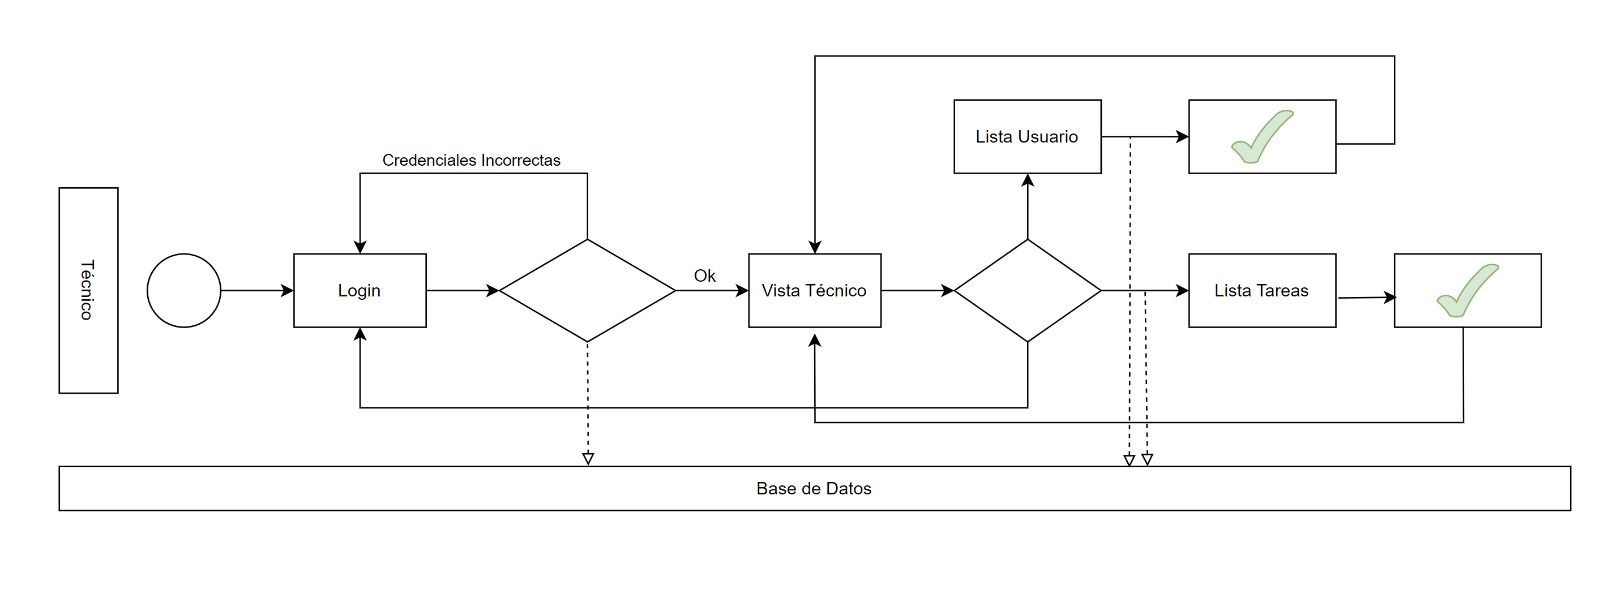
\includegraphics[width=1\textwidth ]{images/procesos_tecnico.jpeg}
	\caption{Diagrama de procesos del técnico}
	\label{fig:example1}
\end{figure}\\


\subsection{Médico}

Al igual que para el técnico, el médico al acceder a la web tiene un inicio de sesión, donde deberá introducir sus credenciales que serán comprobadas en la base de datos. En caso de éxito podrá acceder a la interfaz y sino seguirá en la pestaña de login. Una vez haya accedido a la interfaz de la app, podrá elegir entre diferentes opciones, asignar tareas, notificar una incidencia sobre algún robot, ver la lista de robots o cerrar sesión si así lo desea. En caso de consultar la lista de robots, podrá acceder a una nueva vista con toda la información el robot elegido. En todo momento tras cada vista se harán consultas sobre la base de datos para mostrar información por pantalla o se guardará en la base de datos las incidencias o tareas asignadas.

\begin{figure}[H]
	\centering
	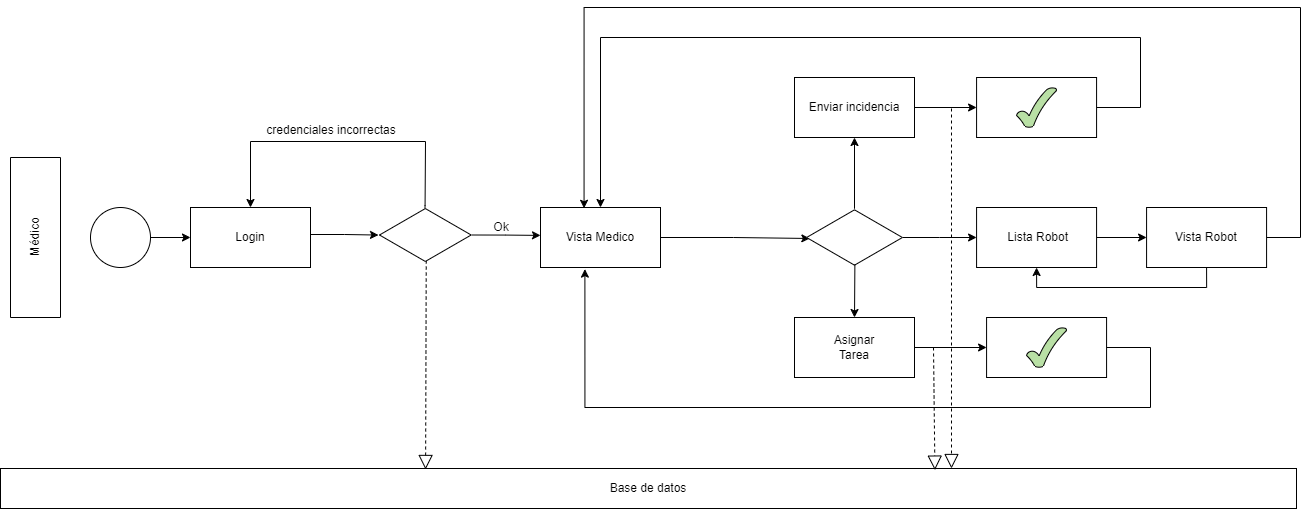
\includegraphics[width=1\textwidth]{images/medico.drawio.png}
	\caption{Diagrama de procesos del médico}
	\label{fig:example1}
\end{figure}

\section{Diagramas IFML}

El lenguaje de \textbf{modelado de flujo de interacción} (IFML) incluye un conjunto de notaciones gráficas para crear modelos visuales de interacciones de usuario y comportamiento de front-end en sistemas de software. \\
\\
Los modelos IFML constan de uno o más contenedores de vista. Estos pueden incluso abarcar otro contenedor de ser necesario, las vistas denotan el contenido estático o dinámico de la página así como los elementos de interfaz para la entrada de datos. Tanto los contenedores como los componentes de una vista se pueden asociar entre si con eventos. Los eventos son situaciones que afectan al estado de la página, la forma de relacionar una vista con una acción es mediante los flujos de navegación que son flechas que nos indican el sentido del flujo.

Algunos beneficios que aporta el desarrollo en IFML:

\begin{itemize}
    \item Permite abordar el modelado desde diferentes perspectivas como son: interfaz, interacción y gestión de eventos.
    \item Aísla los problemas de implementación de front-end con el diseño permitiendo obtener un concepto general del mismo sin preocupaciones.
    \item Mejora la comunicación del diseño de la interfaz de usuario con las partes interesadas no técnicas.
\end{itemize}

\subsection{Técnico} 

Después de iniciar sesión con la cuenta del técnico accedemos a la su interfaz. Desde esta vista podemos elegir entre tres acciones, cada una representada por un botón diferente.La primera opción sería el botón "Incidencias", el cual nos lleva a una nueva vista donde nos saldrá si hay alguna incidencia con algún robot y sus detalles. El siguiente botón que tenemos en la vista principal es "Usuario", este también nos redirige a otra vista donde nos saldrá una lista con los usuarios registrados en el sistema. Desde esta lista podremos eliminar algún usuario existente o registrar algunos nuevos. Para ello usaríamos el botón "UsuarioNuevo" y se nos abriría un formulario donde se introducen los datos para iniciar sesión del nuevo usuario.
La última funcionalidad es "Lista de tareas", este botón nos carga una nueva vista donde veremos una lista con todas las tareas definidas que pueden realizar los robots. Desde esta vista podemos añadir una tarea mediante el formulario que se despliega o pinchar sobre una ya existente, lo que nos llevaría a otra ventana con la tarea elegida y su información.

\begin{figure}[H]
	\centering
	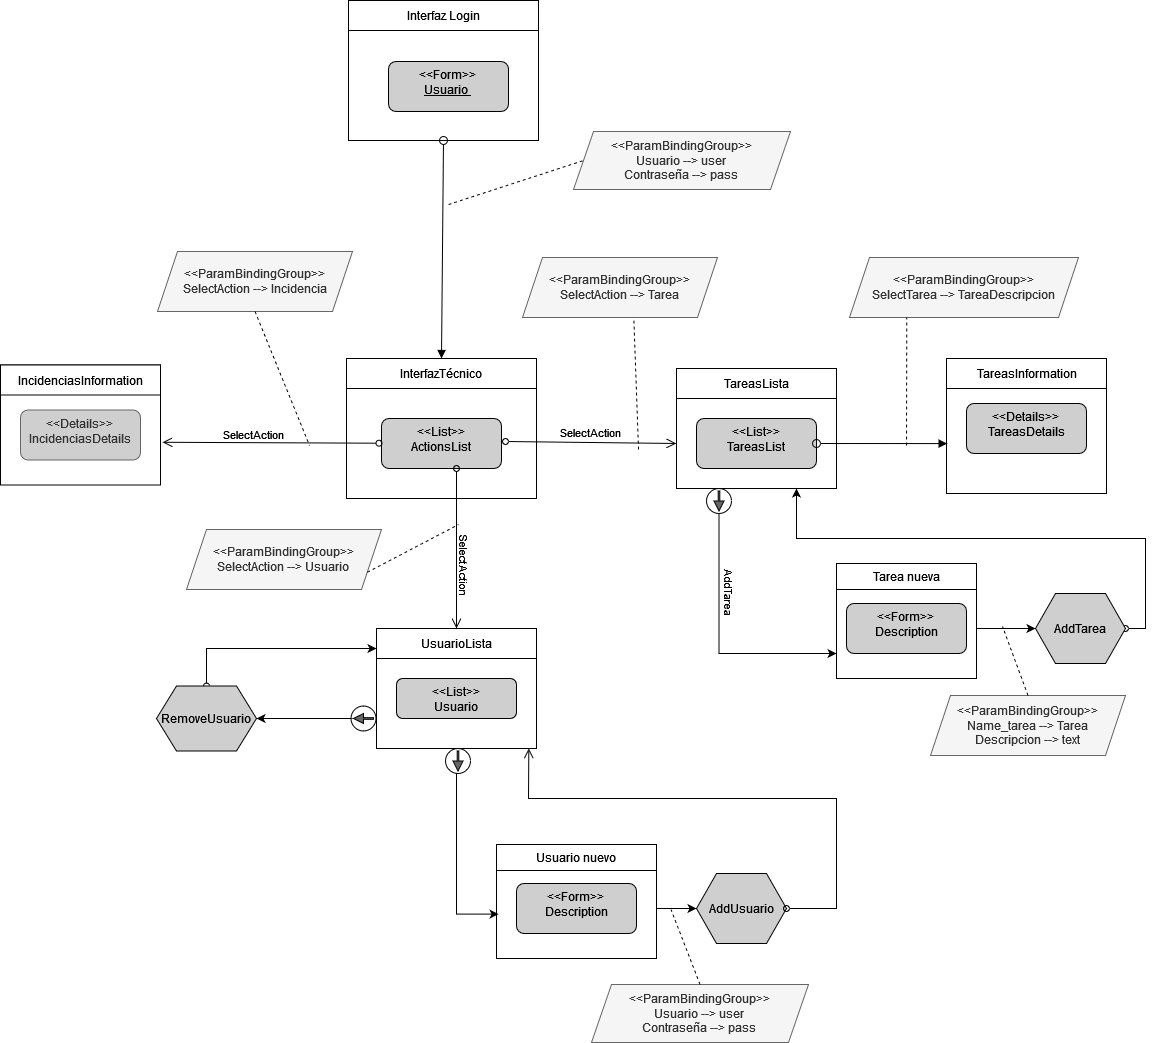
\includegraphics[width=0.9\textwidth]{images/IMFL_tecnico.drawio.png}
	\caption{Diagrama IFML médico}
	\label{fig:example1}
\end{figure}

\newpage

\subsection{Médico} 

Tras hacer login con el usuario y la contraseña del médico accederemos directamente a su interfaz correspondiente. Está es la vista general del médico y en ella aparecen diversos botones, cada botón realiza una función diferente, esto lo podemos observar en el diagrama IFML, dentro del contenedor de interfaz encontramos una \textit{<<List>> ActionList}.Del contenedor salen diferentes flujos de navegación. Leyendo el diagrama de izquierda a derecha la primera funcionalidad de la interfaz de médico que vemos es la de las incidencias. Accedemos a está tras pulsar el botón de enviar incidencias, la vista de las incidencias posee un textbox en el cual el usuario podrá escribir cualquier mensaje que quiera que vea el técnico es por eso que debajo del textbox aparecen dos botones de evento, uno envía el mensaje a la vista del técnico y el otro cancela el proceso devolviéndonos a la interfaz anterior. La segunda funcionalidad es la de asignación de tareas mediante un formulario que aparecerá por pantalla el médico podrá asignar tareas tras asignar o cancelar una tarea volveremos a la interfaz anterior. Por último tenemos la lista de robots donde podremos pinchar en cualquiera de ellos para ver una descripción general de las características del robot.\\
\\

\begin{figure}[H]
	\centering
	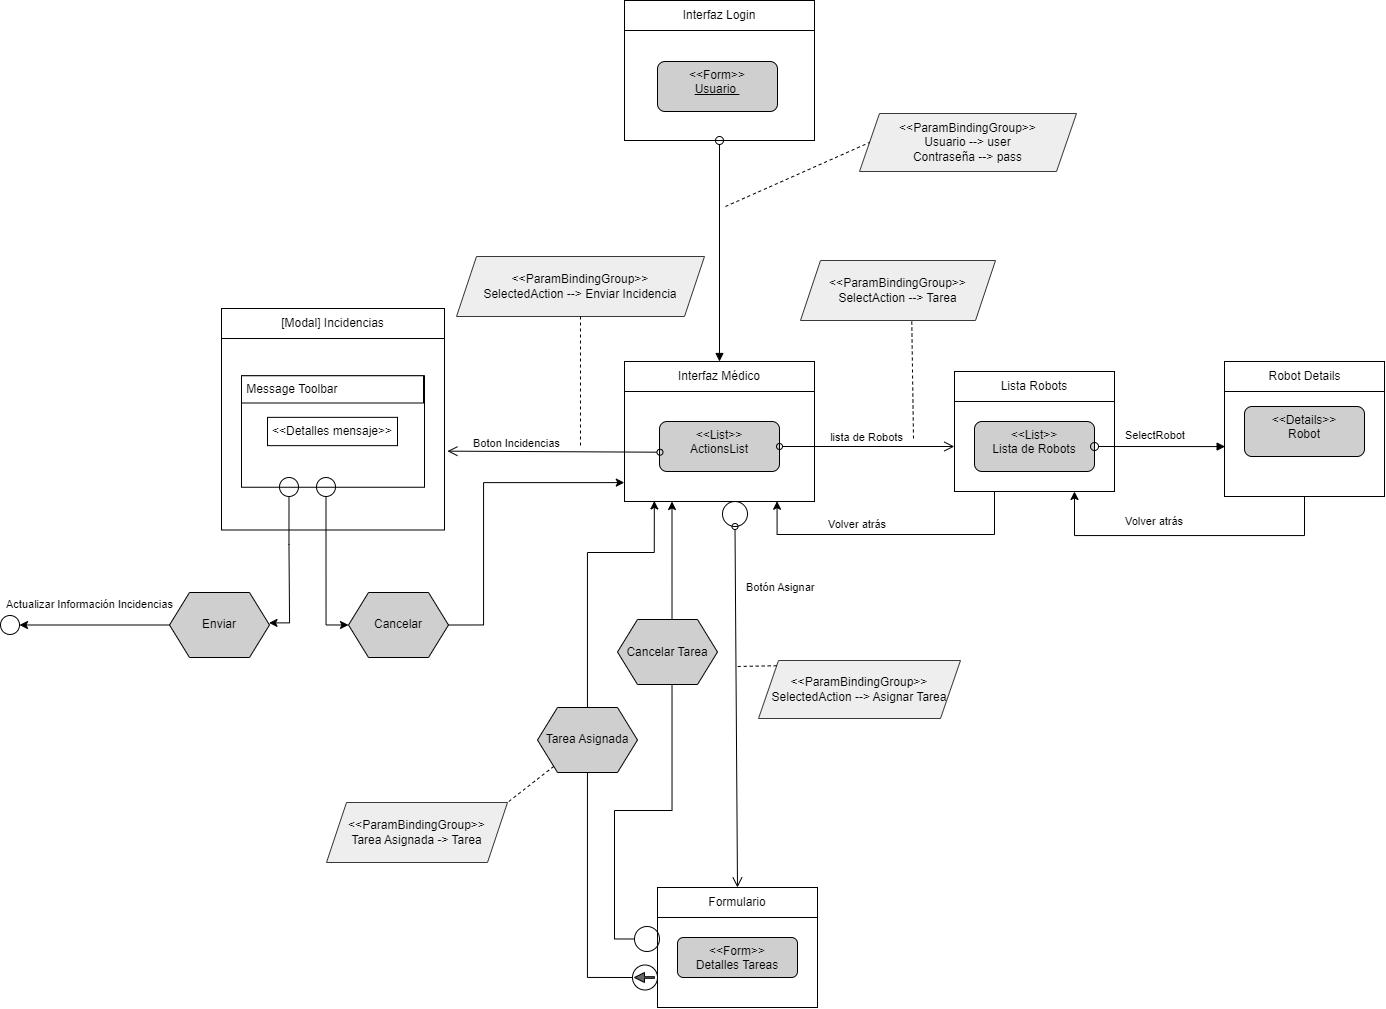
\includegraphics[width=1\textwidth]{images/ifml_medico.drawio.png}
	\caption{Diagrama IFML técnico}
	\label{fig:example1}
\end{figure}


\newpage
\section{Modelado de Contenidos}
En el modelado de contenidos se representa la estructura, el comportamiento y relaciones estáticas de cada uno de los objetos del sistema. \\ \\
El modelo de contenidos esta formado principalmente por los siguientes elementos: \textbf{clases, relaciones e interfaces.} 
\begin{itemize}
    \item Las clases representan entidades u objetos del sistema y tienen atributos y métodos asociados que las definen.
    \item Las relaciones representan como se relacionan los objetos del sistema. Las propiedades definen las relaciones son la multiplicidad(número de elementos que participan en la relación) y el nombre de asociación.
    \item Las interfaces son definidas por una serie de atributos, funciones y obligaciones. Toda clase asociada a una interfaz debe de cumplir con todas aquellas funciones y atributos incluidos en esta.
\end{itemize}  
\vspace{1.5cm}
\begin{figure}[H]
	\centering
    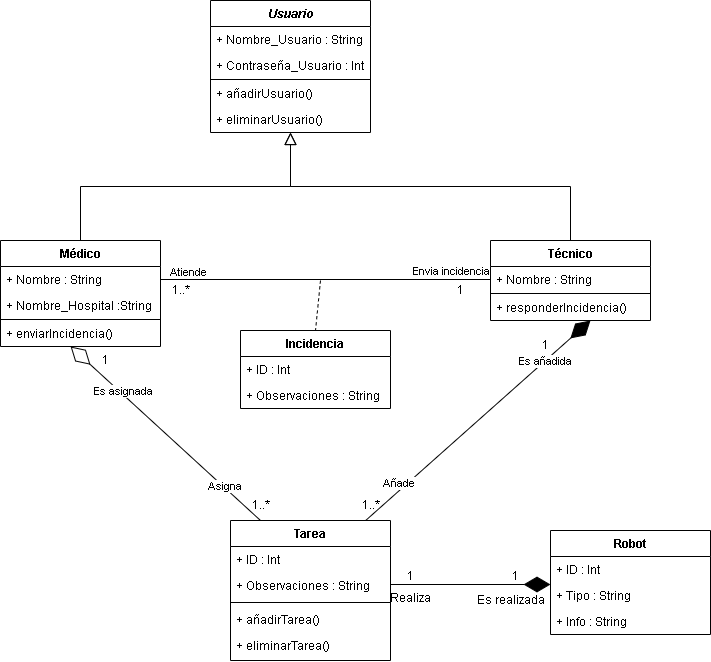
\includegraphics[width=0.75\textwidth]{{images/diagrama-logico-clases.drawio.png}}
	\caption{Modelo de contenidos}
	\label{fig:example1}
\end{figure}

\subsection{Descripción de clases}

\begin{itemize}

    \item \textbf{Clase Usuario:}  Aquellas personas que van hacer uso de la web. Pueden ser médicos o técnicos. 
    \item \textbf{Clase Médico:} Un tipo de usuario. Es el encargado de asignar tareas a los robots y en el caso de incidencias con las plataforma, comunicárselas al técnico. 
    \item \textbf{Clase Técnico:} Un tipo de usuario. Es el encargado de añadir tareas a los robots y atender las incidencias comunicadas por los médicos. 
    \item \textbf{Clase Incidencia:} Modela las incidencias registradas por lo médicos. Dicho objeto almacenas las observaciones realizadas por lo médicos y técnicos.
    \item \textbf{Clase Tarea:} Modela las tareas asignadas y añadidas por los médicos y técnicos respectivamente. Una tarea solo puede ser asignada por un médico. A la vez una tarea solo puede ser añadida por un técnico. Todas las tareas tendrán asignadas un robot que la realice. Una tarea no puede existir sin un técnico que previamente la halla añadido y un robot asociado.
     \item \textbf{Clase Robot:} Modela los robots de la plataforma. Los robots pueden realizar un tipo de tarea.
\end{itemize}

\end{document}